\documentclass[a4paper]{book}

\usepackage[utf8]{inputenc}
\usepackage[german,english,russian]{babel}
\usepackage{hyperref}
\hypersetup{unicode=true}

\usepackage{graphicx}

\title{Стойка ЧПУ KOSY}
\author{перевод Dmitry Ponyatov <dponyatov@gmail.com>}

\begin{document}

\maketitle

Кривой перевод оригинальной документации из поставки учебного комплекта станков
WABECO~--- файлы \verb@nccad7.chm@ и \verb@ZSE3Help.chm@ с немецкого.
Комплектность поставки документации от ecoinvent хромает, могли бы хотя бы
английский вариант положить как опцию.

\tableofcontents

\part{NCCAD7}

% Inhaltsverzeichnis
% Hilfethemen für nccad7 - 18. 02. 2005

% \chapter{Inhaltsverzeichnis} 
\chapter{Suchen von Worten} 

Überarbeitet: August 2002

\bigskip 

Angenommen Sie möchten eine nähere Erklärung zum Begriff "Nullpunkt". Innerhalb aller 
Hilfethemen kommt dieser Begriff auf mehreren Seiten vor. Um diese Seiten - und die 
zugehörigen Textstellen zu finden gibt es die Funktion "Suchen". Sie gehen folgendermaßen 
vor:
\begin{enumerate}
  \item Öffnen Sie die Karteikarte \textbf{Suchen} durch Klick auf den Reiter
  "Suchen".
  \item Geben Sie im \textbf{Feld Suchbegriff} das Suchwort komplett ein. 
\begin{enumerate}
  \item Achten Sie auf Rechtschreibung. 
  \item Die Klein/Großschreibung wird in der Suchfunktion nicht beachtet, z.B.
  \item kann eingegeben werden "nullpunkt" oder "Nullpunkt".
  \item Schon einmal eingegebene Suchworte sind über das PullDown-Menü wieder
  aufrufbar (Pfeil nach unten).
  \item In den Suchbegriff können logische Verknüpfungen eingebaut werden, die
Sie über den Button "Pfeil nach rechts" neben dem Eingabefeld erreichen.
\end{enumerate}
  \item Klicken Sie auf "Themen auflisten". Eine Liste mit den Seiten, in denen
das Suchwort mindestens einmal vorkommt, erscheint.
  \item Wählen Sie durch Doppelklick eine dieser Seiten aus. In der
dargestellten Seite werden die gefundenen Textstellen markiert. Durch Scrollen können Sie die Textstellen auffinden. (Siehe Bild, unterer Teil).
\end{enumerate}

\bigskip

Das folgende Bild gibt einen Überblick über die verschiedenen Phasen des Suchens:

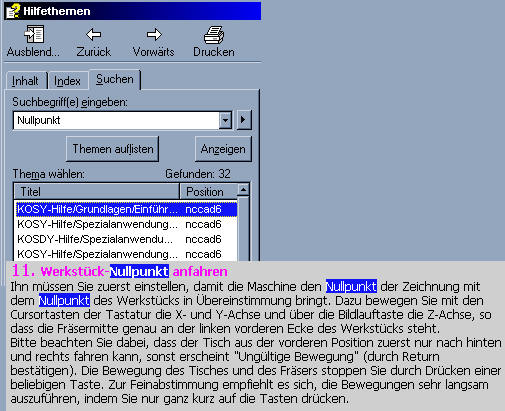
\includegraphics{pic/Suche1.png}

\chapter{Das Indexregister} 
\chapter{Grundlagen der Bedienung} 
	\section{Kurzanleitung}
	\section{Bedienprinzip}
	\section{Drucken}
	\section{Konfiguration von nccad7}
	\section{Vorlagen}
	\section{Das Menü}
		\subsection{Ansicht}
		\subsection{Datei}
		\subsection{Hilfe}
		\subsection{Maschine}
		\subsection{Parameter}
		\subsection{Simulation}
	\section{Die Icons}
		\subsection{Bearbeitung}
			\subsubsection{Drehen}
			\subsubsection{Eigenschaften ändern}
			\subsubsection{Konstruktionspunkt verschieben}
			\subsubsection{Kopieren}
			\subsubsection{Korrektur Texte}
			\subsubsection{Kreisförmig anordnen}
			\subsubsection{Löschen}
			\subsubsection{Löschen Letztes}
			\subsubsection{Rückgängig Letztes}
			\subsubsection{Skalieren}
			\subsubsection{Spiegeln horizontal}
			\subsubsection{Spiegeln horizontal mit Kopie}
			\subsubsection{Spiegeln vertikal}
			\subsubsection{Spiegeln vertikal mit Kopie}
			\subsubsection{Verschieben}
			\subsubsection{Zoom Maßstab}
		\subsection{CAD - 3D}
			\subsubsection{Ansicht dreidimensional}
			\subsubsection{Plastische Zone Kreis}
			\subsubsection{Plastische Zone Rechteck}
			\subsubsection{Plastische Zone in STL wandeln}
			\subsubsection{Schnitt bearbeiten}
			\subsubsection{Schnitt neu}
		\subsection{CAD - Besonderes}
			\subsubsection{Ellipse}
			\subsubsection{Freihand}
			\subsubsection{Kurve Approximation}
			\subsubsection{Kurve Interpolation}
			\subsubsection{Mathematische Funktion}
			\subsubsection{Outline - Generierung}
			\subsubsection{Pad/Bahn - Generierung}
			\subsubsection{Schraffieren}
			\subsubsection{Tangente}
			\subsubsection{Tangente außen}
			\subsubsection{Tangente innen}
			\subsubsection{Zahnrad außenverzahnt}
			\subsubsection{Zahnrad innenverzahnt}
			\subsubsection{Zahnstange}
		\subsection{CAD - Standard}
			\subsubsection{Bogen} 
			\subsubsection{Gerade}
			\subsubsection{Gravurtext MAX/einzeilig} 
			\subsubsection{Gravurtext MAX/mehrzeilig}
			\subsubsection{Gravurtext TrueType} 
			\subsubsection{Kreis} 
			\subsubsection{Langloch} 
			\subsubsection{Polygon} 
			\subsubsection{Polygon-Generierung} 
			\subsubsection{Punkt} 
			\subsubsection{Rechteck} 
		\subsection{CAM - Standard}
			\subsubsection{Ausspannposition} 
			\subsubsection{Bahnkorrektur} 
			\subsubsection{Insel auflösen}
			\subsubsection{Insel zuweisen} 
			\subsubsection{Kontur auflösen}
			\subsubsection{Kontur generieren}
			\subsubsection{Leitkontur} 
			\subsubsection{Tasche fräsen} 
			\subsubsection{Technologie} 
			\subsubsection{Werkstück - Befestigung} 
			\subsubsection{Werkstück - Nullpunkt} 
		\subsection{Darstellung}
			\subsubsection{Ansicht Letzte} 
			\subsubsection{Ausschnitt verschieben} 
			\subsubsection{Ausschnitt wählen} 
			\subsubsection{Neu darstellen} 
			\subsubsection{Tischdarstellung} 
		\subsection{Dokumentation}
			\subsubsection{Bemaßung horizontal} 
			\subsubsection{Bemaßung Radius} 
			\subsubsection{Bemaßung schräg} 
			\subsubsection{Bemaßung vertikal} 
			\subsubsection{Bemaßung Winkel} 
			\subsubsection{Beschriftung TrueType} 
			\subsubsection{Beschriftung MAX/einzeilig} 
			\subsubsection{Beschriftung MAX/mehrzeilig}
			\subsubsection{Bearbeiter} 
			\subsubsection{Bearbeiter letzte Änderung} 
			\subsubsection{Dateiname} 
			\subsubsection{Datum letzte Änderung} 
			\subsubsection{Datum aktuell} 
			\subsubsection{Datum Ausdruck}
			\subsubsection{Datum erstellt} 
		\subsection{Einstellungen}
			\subsubsection{Bezugspunkt} 
			\subsubsection{Fang} 
			\subsubsection{Layer (Zeichnungslage)} 
			\subsubsection{Lineal} 
			\subsubsection{Linien} 
			\subsubsection{Raster} 
		\subsection{Information}
			\subsubsection{Messen} 
			\subsubsection{Zeichnungsteil-Informationen} 
		\subsection{Symbole}
			\subsubsection{Symbol auflösen}
			\subsubsection{Symbol laden} 
			\subsubsection{Symbol speichern} 
		\subsection{Umwandlung}		
			\subsubsection{Trimmen} 
			\subsubsection{Verlängern} 
			\subsubsection{Trimmen-Verlängern} 
			\subsubsection{Trimmen 2 Teile} 
			\subsubsection{Verlängern 2 Teile} 
			\subsubsection{Auftrennen} 
			\subsubsection{Autom. Trimmen-Verl. (Kontur verfolgen)} 
			\subsubsection{Verdünnen} 
			\subsubsection{Polygon-Generierung} 
			\subsubsection{Konvertieren in Gerade} 
			\subsubsection{Konvertieren in Polygon}
			\subsubsection{Runden} 
			\subsubsection{Runden selektiv} 
			\subsubsection{Fasen} 
			\subsubsection{Fasen selektiv} 
						
\chapter{Grundlagen CAD}
	\section{CAD - Konstruktionsgrundlagen}
	\section{CAD - Kurzanleitung}
	\section{CAD - 3D Funktionen}
	\section{CAD - Technisches Zeichnen}
		\subsection{Dreiseiten-Darstellung}
		\subsection{Räumliche Darstellung}
		\subsection{Arbeiten mit Symbolen}
	\section{Grafik}
		\subsection{Bilder importieren}
		\subsection{Formulare}
	 
\chapter{CNC-Fräsmaschinen} 
	\section{Inbetriebnahme, Erste Schritte}
	\section{Handsteuerung}
	\section{CNC-Fräsen}
	\section{Teach In - Programmierung} 
	\section{Simulation mit OpenGL} 
	\section{Werkzeug-Korrektur} 
	\section{CAD/CAM-Fräsen} 
		\subsection{Einführungsbeispiel, Prinzip} 
		\subsection{Technologie-Angaben} 
	\section{3D-Fräsen}
		\subsection{Körper aus Rippen und Spanten} 
		\subsection{Plastische Zonen} 
		\subsection{Randzonen} 
		\subsection{STL Grundlagen} 
		\subsection{STL Ebenenbearbeitung} 
		\subsection{STL 4-Achs-Bearbeitung}
	\section{Bearbeitungseinheiten} 
		\subsection{Universal (Metabo)} 
		\subsection{Schnellfrequenz} 
		\subsection{Drehstrom} 	 
	\section{Arbeitshinweise}
		\subsection{WNP verschieben} 
		\subsection{Maschine aufrüsten}
	\section{Hilfsmittel} 
		\subsection{Pratze, Treppenbock} 
		\subsection{Anschlagwinkel} 		 
	\section{Spezialanwendungen} 
		\subsection{Mit Sonderwerkzeugen}
			\subsubsection{Gewindefräser ZBGF} 
		\subsection{Gravuren} 
			\subsubsection{MAX-Schriften} 
			\subsubsection{TrueType-Schriften} 
			\subsubsection{Fortlaufende Zahlen}
			\subsubsection{am Bogen}
		\subsection{Leiterplatten} 
			\subsubsection{Mit nccad entwerfen und fräsen} 
			\subsubsection{Von Layout-Programmen bearbeiten} 
			\subsubsection{Von Layout-Programmen bohren} 
		\subsection{Zahnräder} 
			\subsubsection{Grundlagen} 
			\subsubsection{Bearbeiten} 
			\subsubsection{Praxis} 			
		\subsection{Schneiden} 
			\subsubsection{Schleppmesser} 
		 
\chapter{CNC-Bohrmaschinen} 
	\section{Bediengrundlagen}

\chapter{CNC-Drehmaschinen}
	\section{Daten und Fakten} 
	\section{Inbetriebnahme, Erste Schritte} 
	\section{CNC-Drehen} 
	\section{Simulation mit OpenGL} 
	\section{Werkzeugverwaltung} 
	\section{Testhilfen} 
	\section{CAD/CAM-Drehen} 
		\subsection{Prinzip} 
		\subsection{Mehrfachzyklen} 
	\section{Spezialanwendungen} 
		\subsection{Gewinde-Drehen} 
		\subsection{CNC-Zyklen} 
 
\chapter{Dosier-Systeme}
	\section{Grundlagen} 
	\section{Schubdosierung} 
 
\chapter{Automatisierungs-Systeme}
	\section{Grundlagen} 
	\section{Schaltfunktionen während Bewegung} 
 
\chapter{KOSY-Steuerungen} 
	\section{Standard-Ausführung} 
	\section{Wabeco-Ausführung} 

\chapter{Spezial-Funktionen/Programme} 
	\section{Hilfsprogramme} 
		\subsection{Zeichensatz-Editor} 

\chapter{Import/Export} 
	\section{CNC-Programmexport} 
	\section{Postprozessoranpassung} 
	\section{Schnittstellen} 
	\section{2D-Import} 
		\subsection{DXF}
		\subsection{HPGL} 
		\subsection{Nachbearbeitung} 
		\subsection{Scannen und Vektorisieren} 
	\section{3D-Import} 
		\subsection{STL}
	\section{3D-Export} 
		\subsection{STL}

\chapter{Optionen und deren Bedienung} 
	\section{Abtasten}
	\section{Drehen} 
	\section{KOSY Wagen} 
	\section{Mindermengendosierung} 
	\section{Schubdosierung} 
	\section{Spooler} 
	\section{Tiefenregelung} 
	\section{Werkzeuglängenmessung} 
	\section{Werkzeugwechsel} 

\chapter{Umgang mit dem System}
	\section{Service und Wartung} 
		\subsection{Fehlerliste} 
		\subsection{Hotline} 
		\subsection{Massiv-Körper reparieren} 
	\section{Transport} 
		\subsection{Massive Maschinen} 
		\subsection{Paketversand} 
 
\chapter{Anhang}
	\section{Liesmich/Installation} 
	\section{Anschlussbelegung} 
	\section{CAM-Technologien} 
	\section{Dreh-Zyklen} 
	\section{NC-Befehle} 
	\section{NC-Kurzbefehlsliste} 
	\section{Netzwerk-Installation} 
	\section{Tastenbelegung (HotKeys)} 
 
 
\part{ZSE3}

\end{document}